\chapter{研究方法}
\section{實驗環境與架構設計}
\begin{figure}[!htbp]
\centering
\scalebox{.35}{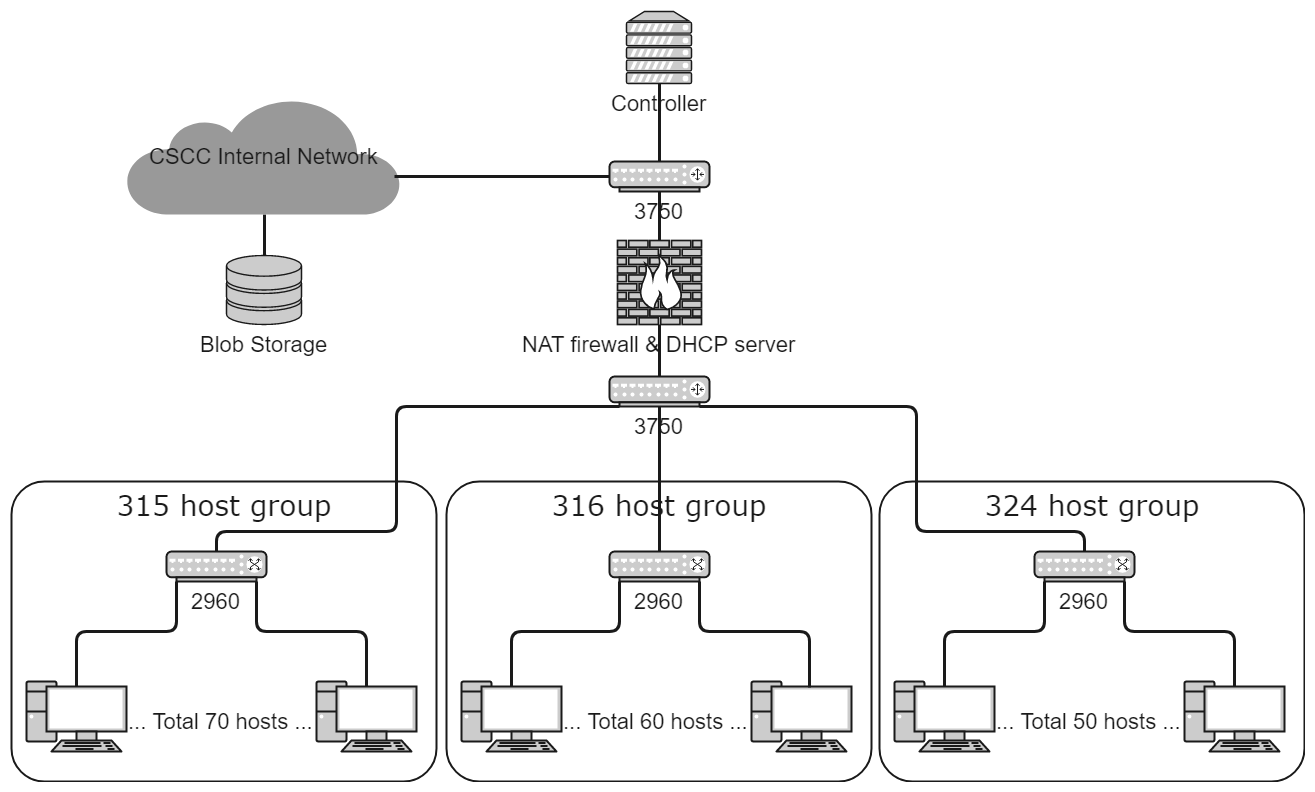
\includegraphics{images/PC_Room_Network.png}}
\caption{PC Room Network.}
\label{i:pcroom}
\end{figure}



在交通大學資訊工程學系計算機中心,需要大量部署 PC 電腦教室 Windows 作業系統與管理。
從圖 \ref{i:pcroom} 可以看見計算機中心有三個主機群,主機數量分別為 50 台在 324 主機群、60 台在 316 主機群、70 台在 315 主機群,總共有 180 台主機需要部署作業系統與組態管理,各主機群的規格如表 \ref{pcspec}。


\begin{table}[htbp]
\centering
\caption{實驗主機群硬體規格}
\label{pcspec}
\begin{adjustbox}{max width=0.92\textwidth}
\begin{tabular}{lrrrrrr}

\toprule
\multicolumn{1}{l}{\textbf{Host Group}} & \textbf{315} & \textbf{316} & \textbf{324} \\ \midrule
\multicolumn{1}{l}{\textbf{Number of Hosts}} & \textbf{70} & \textbf{60} & \textbf{50} \\

\multicolumn{1}{l}{\textbf{CPU}} & \textbf{i5-4570s 2.9GHz} & \textbf{i5-2400s 2.49GHz} & \textbf{i5-7500 3.4GHz} \\

\multicolumn{1}{l}{\textbf{Memory}} & \textbf{4GB DDR3} & \textbf{4GB DDR3} & \textbf{16GB DDR4} \\

\multicolumn{1}{l}{\textbf{HDD}} & \textbf{1TB} & \textbf{500GB} & \textbf{1TB} \\

\multicolumn{1}{l}{\textbf{SSD}} & \textbf{N/A} & \textbf{N/A} & \textbf{250GB} \\

\multicolumn{1}{l}{\textbf{Network Bandwidth}} & \textbf{1Gb/s} & \textbf{1Gb/s} & \textbf{1Gb/s} \\
\bottomrule
\end{tabular}
\end{adjustbox}
\end{table}



以部署系上課程用的映像檔為例,映像檔大小約為 100 GB,若使用三台部署伺服器,各伺服器的硬碟連續讀取速率約為 200 MB/s ,透過一對一的方式傳輸映像檔到所有主機群共 180 台主機,在最佳情況下所需要花費的時間為 512 分鐘。然而一般情況需要考量硬碟隨機讀取速度,且若減少部署伺服器到一台所需時間將倍增為 1536 分鐘,不可能應用在大規模的計算中心。
原先期望透過 Multicast-based 的 Clonezilla Server Edition 加速部署作業,然而其在部署速度和穩定度皆不盡理想。
因此本研究結合了 EZIO ,透過 BitTorrent 協議讓主機間經由對等式網路傳播映像檔,解決部署伺服器硬碟效能瓶頸與網路頻寬利用不足的問題。


此外,由於本研究的目標主機群是一般 PC 主機,並不具備有伺服器管理功能的 IPMI ,因此 BitFission 將透過 Wake-On-Lan、PXE 和 Ansible,進行 Bare-Metal 遠端控制與組態設定。即使沒有 IPMI 遠端管理功能,BitFission 仍可以完成目標主機群的電源控制、自動化部署與組態設定。


本研究將 Bare-Metal Provisioning 區分成以下三個部分:

\begin{enumerate}
\item 裸機再生
\item 映像檔部署
\item 系統組態設定
\end{enumerate}


\section{裸機再生}
\subsection{BitAtom}
\begin{figure}[!htbp]
\centering
\scalebox{.5}{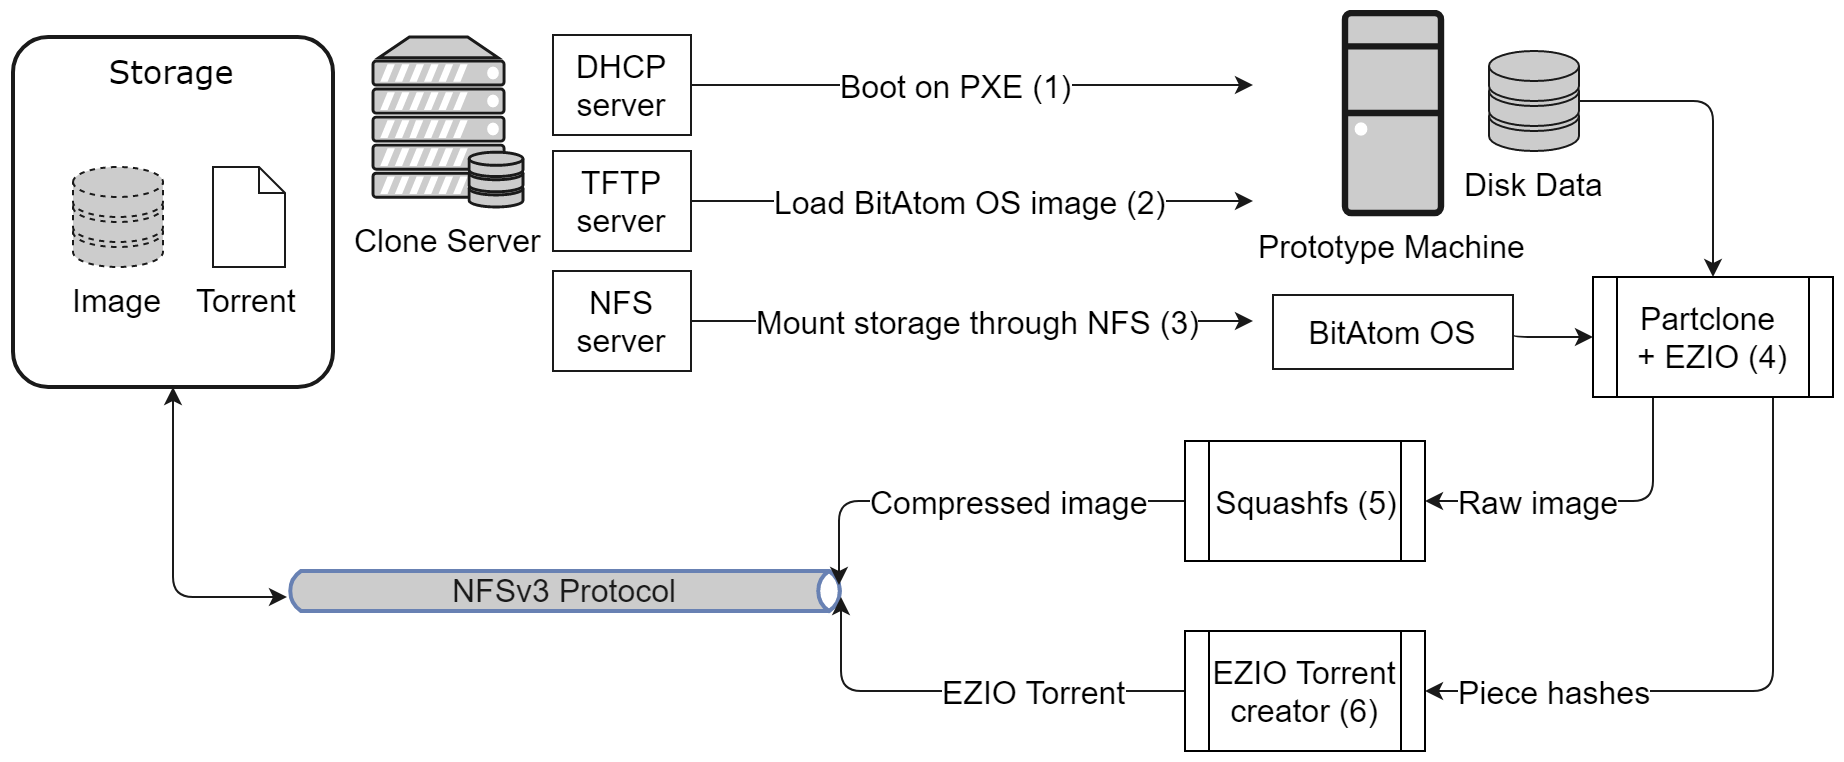
\includegraphics{images/BitAtom_Flowchart.png}}
\caption{BitAtom Flowchart.}
\label{i:bitatomflowchart}
\end{figure}


為了自動化產生映像檔,本研究使用 archiso 客製化了自動備份的特務作業系統 BitAtom,BitAtom 包含 Partclone、NFS client 以及自動化再生映像檔的腳本。
裸機再生流程如圖 \ref{i:bitatomflowchart}。
完整的再生伺服器包含了三項服務(services):DHCP 伺服器、TFTP 伺服器和 NFS 伺服器。
由於原型機本身是電腦教室中的個人電腦,開機時會優先從 PXE 開機,我們將 DHCP 伺服器中的 next-server 指向再生伺服器的 TFTP 伺服器(1),使原型機開機後從 TFTP 上下載 bootloader,再經由 bootloader 載入 TFTP 上的 BitAtom 映像檔(2)。BitAtom 作業系統會依據 TFTP 伺服器上的設定檔或是人工設定進行部署作業,有四項主要設定:
\begin{enumerate}
\item NFS 伺服器 IP 位置
\item NFS 路徑
\item 映像檔儲存路徑
\item 目標再生硬碟
\end{enumerate}
% 我們在再生伺服器上架設 TFTP 伺服器用來提供 BitAtom ISO,並且把 NAT 主機上的 DHCP 伺服器 next-server 選項指向再生伺服器。
% 之後透過 PXE 開機讓原型機從 TFTP 伺服器載入 BitAtom 作業系統映像檔,執行再生腳本將遠端的儲存裝置掛載,隨後透過 Partclone 將原型機的檔案系統轉換成映像檔與種子檔到遠端儲存伺服器。BitAtom 在啟動後會主動嘗試從 TFTP 伺服器下載再生腳本,或是人工設定再生作業,完成設定後就會將再生映像檔自動儲存到儲存伺服器。


\begin{minipage}{\textwidth}
\begin{lstlisting}[caption= The Shell Script of BitAtom]
#!/usr/bin/bash -eu

echo "Type the NFS server IP address or hostname: "
read nfsip
echo "Type target path on the NFS server: "
read nfspath
mount -t nfs ${nfsip}:${nfspath} /mnt

echo "Type the image path e.g. image/win10_20170827 : "
read imgpath
mkdir -p "/mnt/${imgpath}"

while [ 1 ] ; do
echo "Type target disk e.g. sda : "
	read disk
	mkdir -p "/mnt/${imgpath}/${disk}"

	ptype=$(parted /dev/${disk} print | grep "Partition Table:" | cut -d' ' -f 3)
	if [ "${ptype}" == "gpt" ] ; then
		pnum=$(parted -ms /dev/sda print | tail -1| cut -b1)
		gptsize=$(( ${pnum}*128 + 1024 ))
		dd if=/dev/${disk} of=/mnt/${imgpath}/${disk}/partition_table bs=1 count=${gptsize}
	else
		dd if=/dev/${disk} of=/mnt/${imgpath}/${disk}/partition_table bs=1 count=512
	fi

	partitions=$(sfdisk -d /dev/${disk} | grep -e '^/dev/' | cut -d' ' -f1)
	for part in ${partitions}; do
		partclonecmd=""
		fs=$( lsblk -n -f ${part} | cut -d' ' -f2 )
		echo "partition: ${part}. file system: ${fs}."
		if [ "${fs:0:3}" == "ext" ] ; then
			partclonecmd="partclone.extfs -c -a0" 
		# other supported filesystems...
		fi
		mksquashfs /tmp "/mnt/${imgpath}/${disk}/$( printf ${part} | cut -d'/' -f3 ).img" -no-progress -comp lz4 -p "image.img f 444 root root /root/${partclonecmd} -s ${part} -O /dev/stdout | dd bs=4M"
		cat torrent.info | ./partclone_create_torrent.py
		mv /root/a.torrent "/mnt/${imgpath}/${disk}/$( printf ${part} | cut -d'/' -f3 ).torrent"
		rm torrent.info
	done

	echo "Do you want to clone another disk? (y/N)"
	read yorn
	if [ "${yorn}" != "y" ] && [ "${yorn}" != "Y" ] ; then break ; fi
done
\end{lstlisting}
\end{minipage}


\subsection{Partclone}
Partclone 是一個製作分割區映像檔的工具程式,能夠分析檔案系統中的 bitmap,只把分割區中有使用的 block 寫入映像檔中,有效降低映像檔的大小,並且在還原的時候,因為需要讀取跟寫入的資料量減少,提高還原速度。Partclone 支援絕大多數的檔案系統,如 ext2、ext3、ext4、reiserfs、reiser4、xfs、jfs、btrfs、FAT12、FAT16、FAT32、NTFS、HFS、UFS。EZIO 原本也是使用 Partclone 製作映像檔,但是 EZIO 為了支援一般的 BitTorrent 軟體,修改了 Partclone 將每個 block 寫入不同的檔案,產生了許多零碎小檔案且無法進行 Pipe 和壓縮功能,與 Partclone 原生的映像檔相比,占用的硬碟空間超過兩倍以上。
因此本研究決定沿用 Partclone 原生映像檔格式,並且自行開發 BitTorrent 部署軟體解讀 Partclone 原生的映像檔格式,這樣我們便能透過 Pipe 與壓縮,使映像檔的保存更加方便有效率。


\subsection{整合 EZIO 與 Partcone} \label{ezio_and_partclone}
\begin{figure}[!htbp]
\centering
\scalebox{.4}{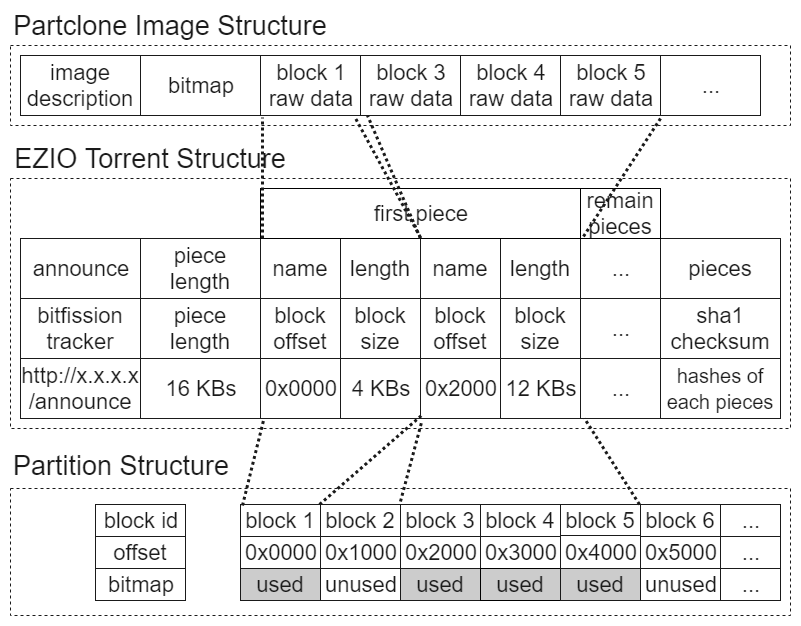
\includegraphics{images/torrent_partition_mapping.png}}
\caption{Torrent Structure.}
\label{i:torrent}
\end{figure}

EZIO 為了能夠把映像檔中每一個 block 正確寫入硬碟上相對應的 offset,我們需要有一個對映映像檔與硬碟分割區的種子檔(torrent) ,同時這個種子檔必須要符合 BitTorrent 協議,才能讓 EZIO 正確解讀。
因此 EZIO 在種子檔上建立了對映表的資訊,如圖\ref{i:torrent}所示,EZIO 將 block 的 offset 作為檔案名稱,以 block 的大小作為檔案長度,並且將連續的 block 合併當作一個檔案提高種子檔的資訊密集度。


為了要產生上述格式的種子檔 ,本研究在 Partclone 備份(Clone)過程中插入製作種子檔的程式碼,當 Partclone 每一次讀取 block 的過程中連帶計算種子檔所需要的雜湊值(pieces checksum) 、block offset 和 block size,如此方法不僅能夠產生種子檔同時也能省去重新讀取硬碟資料的時間。


\subsection{SquashFS}
*TODO 用 Squashfs 和 zstd 進一步解決大型映像檔問題並且能夠些微提高傳輸效率*
*bash 指令*
\begin{table}[!htbp]
\centering
\caption{壓縮演算法比較\cite{zstdbenchmarks}}
\label{t:compressor}
\begin{adjustbox}{max width=0.92\textwidth}
\begin{tabular}{lrrrrrr}

\toprule
\multicolumn{1}{l}{\textbf{壓縮演算法}} & \textbf{壓縮比} & \textbf{壓縮速率} & \textbf{解壓縮速率} \\ \midrule
\multicolumn{1}{l}{\textbf{lz4 1.7.5}} & \textbf{2.101} & \textbf{720MB/s} & \textbf{3600MB/s} \\

\multicolumn{1}{l}{\textbf{zstd 1.1.3-1}} & \textbf{2.877} & \textbf{430MB/s} & \textbf{1110MB/s} \\

\multicolumn{1}{l}{\textbf{zlib 1.2.8-1}} & \textbf{2.743} & \textbf{110MB/s} & \textbf{400MB/s} \\

\multicolumn{1}{l}{\textbf{lzo1x 2.09-1}} & \textbf{2.108} & \textbf{650MB/s} & \textbf{830MB/s} \\

\multicolumn{1}{l}{\textbf{lzf 3.6-1}} & \textbf{2.077} & \textbf{400MB/s} & \textbf{860MB/s} \\

\bottomrule
\end{tabular}
\end{adjustbox}
\end{table}


\section{映像檔部署}
\subsection{BitFission Deployment Server}
1. 如何解決 EZIO 無法支援原生 Partclone image 的問題
2. BT 讓架構簡單化,不需要複雜的 infra 技術或是 SA 
3. 流程圖
\begin{figure}[!htbp]
\centering
\scalebox{.24}{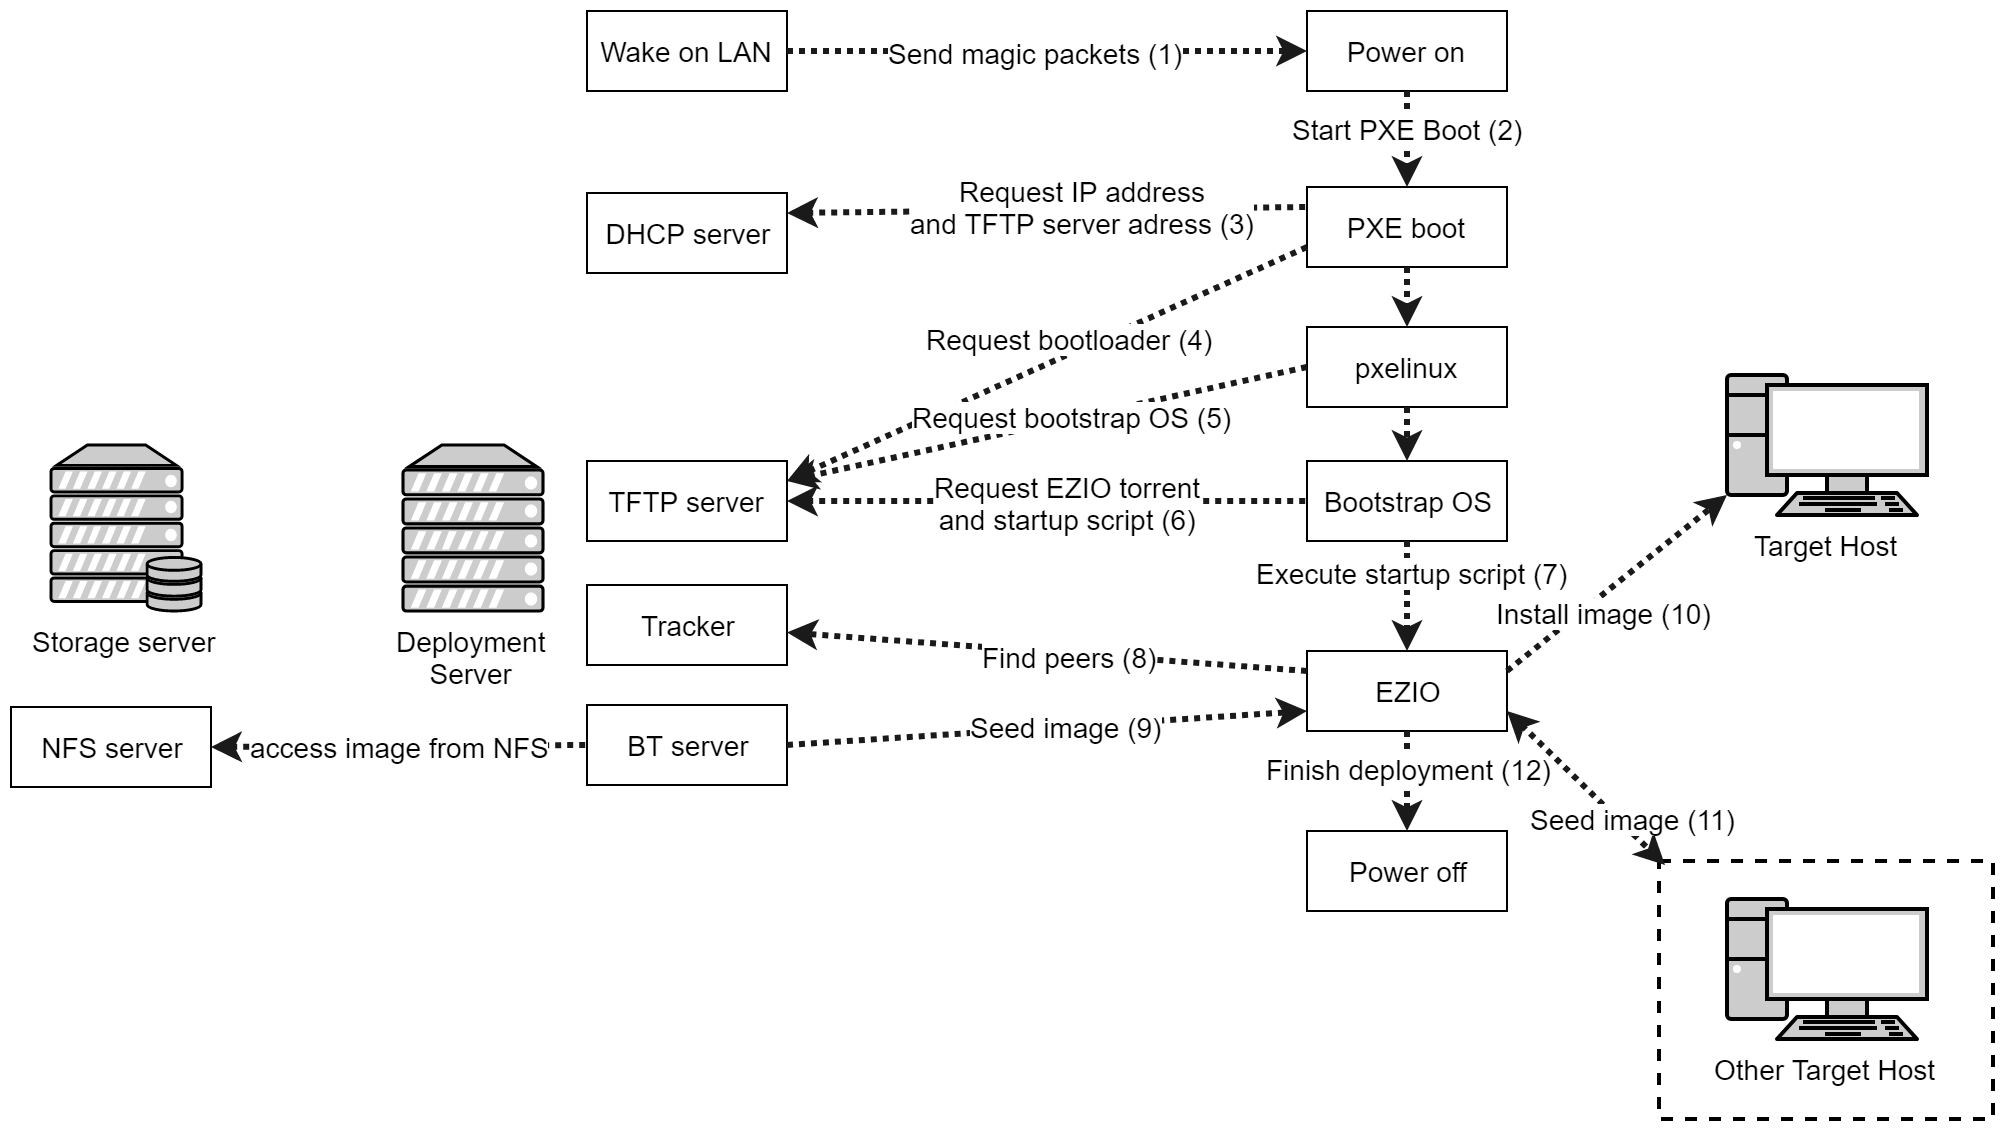
\includegraphics{images/BitFission_Deploy_Flowchart.png}}
\caption{BitFission Deployment Flowchart.}
\label{i:bitfissionflowchart}
\end{figure}


在部署前有幾點問題需要解決。
首先 EZIO 原先的映像檔是自製的規格無法兼容於 Partclone 原生的映像檔,因此 BitFission 的部署伺服器必須要當兩者之間的橋樑,本研究在部署程式中透過映像檔的 bitmap 將 piece 的 offset 轉換成映像檔的 offset 後,在從映像檔中讀取資料並且傳輸給 EZIO 的 BT 客戶端,如圖 \ref{i:flowchart} 所示,只要從映像檔讀取正確的 piece 並傳輸給 EZIO BitTorrent client 就可以還原硬碟資料。
第二,BT 下載者與上傳者需要透過 tracker 傳遞資訊才能連結彼此,因此 BitFission 使用 Opentracker 架設 tracker 服務,並且可以利用 Opentracker 平均分布流量,避免下載者全部擠向同一個上傳者。第三,如何讓客戶端載入 ezio 系統

\begin{minipage}{\textwidth}
\begin{lstlisting}[caption={The Shell Script of BitFission Server}]
#!/usr/bin/bash -eu

scriptpath="$(dirname "$0")"

source "${scriptpath}/dialog.sh"
source "${scriptpath}/network.sh"
if [ -z "${ipaddr-}" ] ; then
	msgbox "Could not get an IP address."
	exit 1
fi

source "${scriptpath}/storage.sh"
if [ -z "${fullpath-}" ] ; then
	msgbox "Could not get the image path."
	exit 1
fi

echo -n "" > torrent.list
while true ; do
	inputbox "Type target disk e.g. sda" "disk"
	mkdir -p /tmp/bitfission/"${disk}"
	mkdir -p /srv/tftp/ezio/"${disk}"
	cp "${fullpath}"/"${disk}"/partition_table /srv/tftp/ezio/"${disk}"/"${disk}"_partition_table
	partitions=$( find "${fullpath}"/"${disk}"/ -name "*.img" | sed -e 's/.*\/\(.*\)\.img/\1/' )
	for part in ${partitions}; do
		mkdir -p /tmp/bitfission/"${disk}"/"${part}"/
		cp "${fullpath}"/"${disk}"/"${part}".torrent /srv/tftp/ezio/"${disk}"/"${part}".torrent
		transmission-edit -a "http://""${ipaddr}"":6969/announce" /srv/tftp/ezio/"${disk}"/"${part}".torrent &>/dev/null
		mount -t squashfs "${fullpath}"/"${disk}"/"${part}".img /tmp/bitfission/"${disk}"/"${part}"/
		offset=$( /usr/local/bin/partclone.info /tmp/bitfission/"${disk}"/"${part}"/image.img 2>/dev/null | cut -d ' ' -f4 )
		if [[ -z "${offset}" ]] ; then offset="0" ; fi
		echo "${offset} /tmp/bitfission/${disk}/${part}/image.img /srv/tftp/ezio/${disk}/${part}.torrent" >> torrent.list
	done
	dialog --yesno "Do you want to clone another disk? (y/N)" 0 0 || break
done

create_ezio_config.sh
chmod a+r -R /srv/tftp/ezio/
killall -p opentracker &>/dev/null || true
opentracker &
bt_server -l torrent.list
\end{lstlisting}
\end{minipage}


\subsection{EZIO}
二〇一七年,由臺灣國立交通大學研究生黃宇強和顏靖軒共同的開發基於 BitTorrent 協議的硬碟部署軟體 EZIO\cite{ezio} 透過 libtorrent 函式庫實作了 BitTorrent-based broadcast 硬碟部署方法。由於 BitTorrent 協議的去中心化設計,透過 peer-to-peer 傳輸檔案有效利用每個主機節點的硬體資源,使得效率接近 Multicast ,在實際的應用下甚至勝過 Multicast 。且 BitTorrent 協議具備非同步的特性,部署時不受單一主機異常而影響其他主機,異常主機也可以在一定時間內重新回到部署作業中。而 EZIO 使用了當中最成熟的 libtorrent 函式庫作為 EZIO 的開發基底,效能比起其他 BitTorrent 函式庫更好。此外,由於 BitTorrent 協議的 resume 功能,使得部署作業得以僅還原硬碟與映像檔有差異的片段(piece),進行差異式部署降低硬碟寫入次數與網路傳輸量。對於使用同一基礎映像檔(base Image)產生的差異映像檔(differential Image),可以提高部署效率並減少硬碟寫入次數。綜合上述 EZIO 與 BitTorrent 的特性,本研究認為 EZIO 適合作為部署程式的載體,再由 BitFission 提供額外的輔助機制便能達成自動化部署。

\subsection{BT Server}
\begin{figure}[!htbp]
\centering
\scalebox{.56}{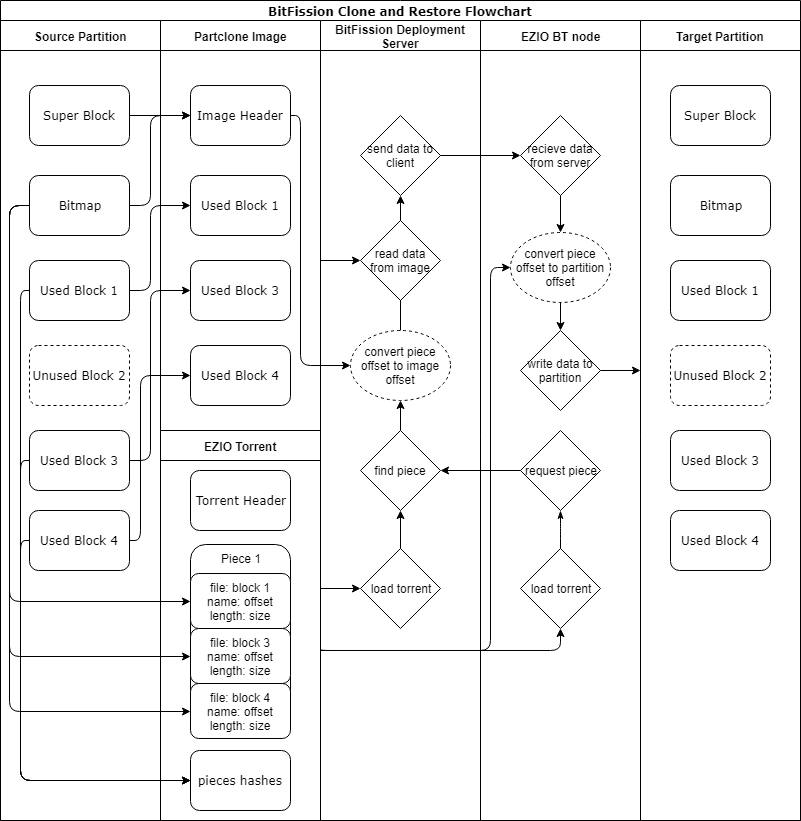
\includegraphics{images/BitFission_Clone_Flowchart.png}}
\caption{BitFission Flowchart.}
\label{i:flowchart}
\end{figure}

在圖 \ref{i:bitfissionflowchart} 中,BT Server 用以作為 BitTorrent 協議的播種伺服器(seeding server),是 BitFission 對等式網路部署的映像檔源頭。
由於要整合 EZIO 和 Partclone 的映像檔 [\ref{ezio_and_partclone}] ,我們不能使用無法解析 Partclone 映像檔格式的一般BitTorrent 軟體,因此本研究使用 libtorrent 函式庫自行撰寫了能夠讀取 Partclone 映像檔的 BT Server。

圖 \ref{i:flowchart} 是 BT Server 與 EZIO 溝通的流程圖,BT Server 與 EZIO 皆載入由 Partclone 產生的 EZIO 種子檔,由 EZIO 發送片段請求給 BT Server,BT Server 解讀種子檔與 Partclone 映像檔後,回傳對應的片段至 EZIO,EZIO 在將之寫入硬碟之中。

原始碼 \ref{readv} 是 BT Server 中解讀 Partclone 映像檔格式的函式 readv,readv 是 libtorrent storage\_interface 中讀取來源檔案的函式,本研究透過 overwrite readv 函式來讀取映像檔。
在第21行可以看到如何計算 EZIO 片段與Partclone 映像檔區塊的對應。
首先映像檔本身包含標頭檔(header),我們需要偏移標頭檔大小,即 image\_head\_size。
再者是 libtorrent 讀取當前片段(piece)的偏移,即 offset。最後是先前片段的長度總和,即 piece*piece\_length()。
三者總和便是 libtorrent 讀取所需片段在 Partclone 映像檔上需要偏移的長度。

\begin{minipage}{\textwidth}
\begin{lstlisting}[label={readv},caption={readv function of BT Server},language=c]
int readv(lt::file::iovec_t const* bufs, int num_bufs, int piece, int offset, int flags, lt::storage_error& ec)
	{
		int index = 0;
		int i = 0;
		int ret = 0;
		unsigned long long device_offset = 0;
		unsigned long long fd_offset = 0; // A fd' point we read data from fd from 
		unsigned long long cur_offset = 0; // A pieces' point we have to write data until
		unsigned long long remain_len = 0;
		unsigned long long piece_sum = 0;
		unsigned long long data_len = 0;
		char *data_buf, *data_ptr = NULL;
		char filename[33]; // Should be the max length of file name
		
		// Caculate the length of all bufs
		for( i = 0 ; i < num_bufs ; i ++){
			data_len += bufs[i].iov_len;
		}
		data_buf = (char *)malloc(data_len);
		
		fd_offset = image_head_size + offset + piece * std::uint64_t(m_files.piece_length());
		ret = pread(this->fd, data_buf, data_len, fd_offset);
		// Copy data_buf to bufs
		data_ptr = data_buf;
		for( i = 0 ; i < num_bufs ; i ++){
			memcpy(bufs[i].iov_base, data_ptr, bufs[i].iov_len);
			data_ptr += bufs[i].iov_len;
		}
		free(data_buf);
		return ret;
	}
\end{lstlisting}
\end{minipage}


\subsection{Tracker}

\section{系統組態設定}
依前面章節所述,如今組態管理工具已發展成熟,本研究採用既有的工具開發 BitFission 的組態管理系統。
而組態管理的方式可分為推播式或拉取式,本研究在兩者中各取其一做比較,並以此決定使用哪種模式的工具。


綜合以上考量,本研究決定採用推播式的 Ansible 作為 BitFission 的組態管理系統核心。

